%---- IMPORTANTE ----
% Esta plantilla está basada en las recomendaciones de la guía "Trabajo fin de Grado: Escribir el TFG", que encontrarás en http://uc3m.libguides.com/TFG/escribir
% contiene recomendaciones de la Biblioteca basadas principalmente en estilos APA e IEEE, pero debes seguir siempre las orientaciones de tu Tutor de TFG y la normativa de TFG para tu titulación.
% Encontrarás un ejemplo de TFG realizado con esta misma plantilla en el archivo "ejemplo_TFG_2017.zip", incluido en la misma carpeta. Consúltalo porque contiene ejemplos útiles para incorporar tablas, figuras, listados de código, bibliografía, etc.


%----------
%	CONFIGURACIÓN DEL DOCUMENTO
%----------

\documentclass[12pt]{report} %fuente a 12pt

% MÁRGENES: 2,5 cm sup. e inf.; 3 cm izdo. y dcho.
\usepackage[
a4paper,
vmargin=2.5cm,
hmargin=3cm
]{geometry}

% INTERLINEADO: Estrecho (6 ptos./interlineado 1,15) o Moderado (6 ptos./interlineado 1,5)
\renewcommand{\baselinestretch}{1.15}
\parskip=6pt

% soporte para generar PDF/A --es importante de cara a su inclusión en e-Archivo porque es el formato óptimo de preservación y a la generación de metadatos, tal y como se describe en http://uc3m.libguides.com/ld.php?content_id=31389625. En la carpeta incluímos el archivo plantilla_tfg_2017.xmpdata en el que puedes incluir los metadatos que se incorporarán al archivo PDF cuando lo compiles. Ese archivo debe llamarse igual que tu archivo .tex
\usepackage[a-1b]{pdfx}

\usepackage{hyperref}
\hypersetup{linktoc=all}

% Expresiones matemáticas
\usepackage{amsmath,amssymb,amsfonts,amsthm}

\usepackage{txfonts} 
\usepackage[T1]{fontenc}
\usepackage[utf8]{inputenc}

\usepackage[spanish, es-tabla]{babel} % información sobre el paquete babel para español http://osl.ugr.es/CTAN/language/spanish/babel/base/spanish.pdf
\usepackage[babel, spanish=spanish]{csquotes}
\AtBeginEnvironment{quote}{\small}

% DEFINICIÓN DE COLORES para portada y listados de código
\usepackage{color}
\definecolor{azulUC3M}{RGB}{0,0,102}
\definecolor{gray97}{gray}{.97}
\definecolor{gray75}{gray}{.75}
\definecolor{gray45}{gray}{.45}

% diseño de PIE DE PÁGINA
\usepackage{fancyhdr}
\pagestyle{fancy}
\fancyhf{}
\renewcommand{\headrulewidth}{0pt}
\rfoot{\thepage}
\fancypagestyle{plain}{\pagestyle{fancy}}

% DISEÑO DE LOS TÍTULOS de las partes del trabajo (capítulos y epígrafes o subcapítulos)
\usepackage{titlesec}
\usepackage{titletoc}
\titleformat{\chapter}[block]
	{\large\bfseries\filcenter}
	{\thechapter.}
	{5pt}
	{\MakeUppercase}
	{}
\titlespacing{\chapter}{0pt}{0pt}{*3}
\titlecontents{chapter}
	[0pt]                                               
	{}
	{\contentsmargin{0pt}\thecontentslabel.\enspace\uppercase}
	{\contentsmargin{0pt}\uppercase}                        
	{\titlerule*[.7pc]{.}\contentspage}                 
  
\titleformat{\section}
	{\bfseries}
	{\thesection.}
	{5pt}
	{}
\titlecontents{section}
	[5pt]                                               
	{}
	{\contentsmargin{0pt}\thecontentslabel.\enspace}
	{\contentsmargin{0pt}}
	{\titlerule*[.7pc]{.}\contentspage}

\titleformat{\subsection}
	{\normalsize\bfseries}
	{\thesubsection.}
	{5pt}
	{}
\titlecontents{subsection}
	[10pt]                                               
	{}
	{\contentsmargin{0pt}                          
		\thecontentslabel.\enspace}
	{\contentsmargin{0pt}}                        
	{\titlerule*[.7pc]{.}\contentspage}  


% DISEÑO DE TABLAS. Puedes elegir entre el estilo para ingeniería o para ciencias sociales y humanidades. Por defecto, está activado el estilo de ingeniería. Si deseas utilizar el otro, comenta las líneas del diseño de ingeniería y descomenta las del diseño de ciencias sociales y humanidades
\usepackage{multirow} % permite combinar celdas 
\usepackage{caption} % para personalizar el título de tablas y figuras
\usepackage{floatrow} % utilizamos este paquete y sus macros \ttabbox y \ffigbox para alinear los nombres de tablas y figuras de acuerdo con el estilo definido. Para su uso ver archivo de ejemplo 
\usepackage{array} % con este paquete podemos definir en la siguiente línea un nuevo tipo de columna para tablas: ancho personalizado y contenido centrado
\newcolumntype{P}[1]{>{\centering\arraybackslash}p{#1}}
\DeclareCaptionFormat{upper}{#1#2\uppercase{#3}\par}

% Diseño de tabla para ingeniería
\captionsetup[table]{
	format=upper,
	name=TABLA,
	justification=centering,
	labelsep=period,
	width=.75\linewidth,
	labelfont=small,
	font=small,
}

%Diseño de tabla para ciencias sociales y humanidades
%\captionsetup[table]{
%	justification=raggedright,
%	labelsep=period,
%	labelfont=small,
%	singlelinecheck=false,
%	font={small,bf}
%}


% DISEÑO DE FIGURAS. Puedes elegir entre el estilo para ingeniería o para ciencias sociales y humanidades. Por defecto, está activado el estilo de ingeniería. Si deseas utilizar el otro, comenta las líneas del diseño de ingeniería y descomenta las del diseño de ciencias sociales y humanidades
\usepackage{graphicx}
\graphicspath{{imagenes/}} %ruta a la carpeta de imágenes

% Diseño de figuras para ingeniería
\captionsetup[figure]{
	format=hang,
	name=Fig.,
	singlelinecheck=off,
	labelsep=period,
	labelfont=small,
	font=small		
}

% Diseño de figuras para ciencias sociales y humanidades
%\captionsetup[figure]{
%	format=hang,
%	name=Figura,
%	singlelinecheck=off,
%	labelsep=period,
%	labelfont=small,
%	font=small		
%}


% NOTAS A PIE DE PÁGINA
\usepackage{chngcntr} %para numeración contínua de las notas al pie
\counterwithout{footnote}{chapter}

% LISTADOS DE CÓDIGO
% soporte y estilo para listados de código. Más información en https://es.wikibooks.org/wiki/Manual_de_LaTeX/Listados_de_código/Listados_con_listings
\usepackage{listings}

% definimos un estilo de listings
\lstdefinestyle{estilo}{ frame=Ltb,
	framerule=0pt,
	aboveskip=0.5cm,
	framextopmargin=3pt,
	framexbottommargin=3pt,
	framexleftmargin=0.4cm,
	framesep=0pt,
	rulesep=.4pt,
	backgroundcolor=\color{gray97},
	rulesepcolor=\color{black},
	%
	basicstyle=\ttfamily\footnotesize,
	keywordstyle=\bfseries,
	stringstyle=\ttfamily,
	showstringspaces = false,
	commentstyle=\color{gray45},     
	%
	numbers=left,
	numbersep=15pt,
	numberstyle=\tiny,
	numberfirstline = false,
	breaklines=true,
	xleftmargin=\parindent
}

\captionsetup[lstlisting]{font=small, labelsep=period}
% fijamos el estilo a utilizar 
\lstset{style=estilo}
\renewcommand{\lstlistingname}{\uppercase{Código}}


%BIBLIOGRAFÍA - PUEDES ELEGIR ENTRE ESTILO IEEE O APA. POR DEFECTO ESTÁ CONFIGURADO IEEE. SI DESEAS USAR APA, COMENTA LAS LÍNEA DE IEEE Y DESCOMENTA LAS DE APA. Si haces cambios en la configuración de la bibliografía y no obtienes los resultados esperados, es recomendable limpiar los archivos auxiliares y volver a compilar en este orden: COMPILAR-BIBLIOGRAFIA-COMPILAR
% Tienes más información sobre cómo generar bibliografía en http://tex.stackexchange.com/questions/154751/biblatex-with-biber-configuring-my-editor-to-avoid-undefined-citations , https://es.sharelatex.com/learn/Bibliography_management_in_LaTeX y en http://www.ctan.org/tex-archive/macros/latex/exptl/biblatex-contrib
% También te recomendamos consultar la guía temática de la Biblioteca sobre citas bibliográficas: http://uc3m.libguides.com/guias_tematicas/citas_bibliograficas/inicio

% CONFIGURACIÓN PARA LA BIBLIOGRAFÍA IEEE
\usepackage[backend=bibtex, style=ieee, isbn=false,sortcites, maxbibnames=5, minbibnames=1]{biblatex} % Configuración para el estilo de citas de IEEE, recomendado para el área de ingeniería. "maxbibnames" indica que a partir de 5 autores trunque la lista el primero (minbibnames) y añada "et al." tal y como se utiliza en el estilo IEEE.

%CONFIGURACIÓN PARA LA BIBLIOGRAFÍA APA
%\usepackage[style=apa, backend=biber, natbib=true, hyperref=true, uniquelist=false, sortcites]{biblatex}
%\DeclareLanguageMapping{spanish}{spanish-apa}

% Añadimos las siguientes indicaciones para mejorar la adaptación de los estilos en español
\DefineBibliographyStrings{spanish}{%
	andothers = {et\addabbrvspace al\adddot}
}
\DefineBibliographyStrings{spanish}{
	url = {\adddot\space[En línea]\adddot\space Disponible en:}
}
\DefineBibliographyStrings{spanish}{
	urlseen = {Acceso:}
}
\DefineBibliographyStrings{spanish}{
	pages = {pp\adddot},
	page = {p.\adddot}
}

\addbibresource{bibliografia/bibliografia.bib} % llama al archivo bibliografia.bib que utilizamos de ejemplo


%-------------
%	DOCUMENTO
%-------------

\begin{document}
\pagenumbering{roman}
	
%----------
%	PORTADA
%----------	
\begin{titlepage}
	\begin{sffamily}
	\color{azulUC3M}
	\begin{center}
		\begin{figure}[H] %incluimos el logotipo de la Universidad
			\makebox[\textwidth][c]{
\includegraphics[width=16cm]{Portada_Logo.png}}
		\end{figure}
		\vspace{2.5cm}
		\begin{Large}
			Grado Ingeniería de Sistemas Audiovisuales\\			
			2018-2019\\
			\vspace{2cm}		
			\textsl{Trabajo Fin de Grado}
			\bigskip
			
		\end{Large}
		 	{\Huge ``Diseño e implementación de un microservicio con Spring''}\\
		 	\vspace*{0.5cm}
	 		\rule{10.5cm}{0.1mm}\\
			\vspace*{0.9cm}
			{\LARGE Jesús Rienda Iáñez}\\ 
			\vspace*{1cm}
		\begin{Large}
			Tutor/es\\
			Carmen Pelaez Moreno\\
			Leganés, 2019\\
		\end{Large}
	\end{center}
	\vfill
	\color{black}
	
\includegraphics[width=4.2cm]{imagenes/creativecommons.png}\\
	\emph{[Incluir en el caso del interés en su publicación en el archivo abierto]}\\
	Esta obra se encuentra sujeta a la licencia Creative Commons \textbf{Reconocimiento - No Comercial - Sin Obra Derivada}
	\end{sffamily}
\end{titlepage}

\newpage %página en blanco o de cortesía
\thispagestyle{empty}
\mbox{}

%----------
%	RESUMEN Y PALABRAS CLAVE
%----------	
\renewcommand\abstractname{\large\bfseries\filcenter\uppercase{Resumen}}
\begin{abstract}
\thispagestyle{plain}
\setcounter{page}{3}
	
	% ESCRIBIR EL RESUMEN AQUÍ
	
	\textbf{Palabras clave:}
	% Escribir las palabras clave aquí
	
	\vfill
\end{abstract}
	\newpage %página en blanco o de cortesía
	\thispagestyle{empty}
	\mbox{}


%----------
%	DEDICATORIA
%----------	
\chapter*{Dedicatoria}

\setcounter{page}{5}
	
	% ESCRIBIR LA DEDICATORIA AQUÍ	
		
	\vfill
	
	\newpage %página en blanco o de cortesía
	\thispagestyle{empty}
	\mbox{}
	

%----------
%	ÍNDICES
%----------	

%--
%Índice general
%-
\tableofcontents
\thispagestyle{fancy}

\newpage %página en blanco o de cortesía
\thispagestyle{empty}
\mbox{}

%--
%Índice de figuras. Si no se incluyen, comenta las líneas siguientes
%-
\listoffigures
\thispagestyle{fancy}

\newpage %página en blanco o de cortesía
\thispagestyle{empty}
\mbox{}

%--
%Índice de tablas. Si no se incluyen, comenta las líneas siguientes
%-
\listoftables
\thispagestyle{fancy}

\newpage %página en blanco o de cortesía
\thispagestyle{empty}
\mbox{}


%----------
%	TRABAJO
%----------	
\clearpage
\pagenumbering{arabic} % numeración con múmeros arábigos para el resto de la publicación	

\chapter{Introducción}

	% COMENZAR A ESCRIBIR EL TRABAJO
	
	\section{Planteamiento del problema}
	Tenemos la necesidad almacenar una serie de datos en una base da datos para posteriormente consultarlos, actualizarlos o crear nuevos registros. Por lo que necesitamos crear un servicio que cuando llamemos nos devuelva los datos almacenados con un tratamiento especifico y un formato definido. Necesitamos que sea sencillo y simple para el cliente que va a consumir dicho servicio. 
	Este servicio tendrá que tener una alta disponibilidad y escalarse cuando sea necesario para siempre tener unos tiempos de respuesta bajos.
	\section{Solución propuesta}
	Para poder resolver nuestro problema usaremos un protocolo REST para la transferencia de datos entre el servicio y el cliente. El servicio web sera un microservicio desarrollado con Spring Boot. En cuanto a la base de datos utilizaremos una base de datos PostgreSQL.
	\section{Justificacion de la solucion}
	
	La arquitectura de microservicios pretende dividir una aplicación compleja en pequeños servicios que solo realicen una función especifica y se comuniquen entre ellos para formar la aplicación final.
	
	Cada microservico es totalmente independiente de desarrollar frente al conjunto, lo cual nos viene genial ya que nuestra idea es realizar una pequeña aplicación que aceda a una base de datos y en un futuro ampliar a varias aplicaciones o incluso un frontal. Los microservicios nos permiten desarrollar cada una en un lenguaje de programación diferente.
	
	Al no disponer de una maquina donde desplegar la aplicación, es ideal que los microservicios lleven un servidor de despliegue(tomcat) embebido y así desplegar en la nube dentro de un contenedor de aplicaciones.
	
	Una vez desplegado en la nube decidimos que la comunicación sería mediante REST ya que es un protocolo simple y muy eficaz para realizar las distintas operaciones(verbos) en base de datos: añadir, recuperar, actualizar y eliminar, esto en REST seria GET, POST, PUT y DELETE.
	
	En cuanto a base de datos hemos elegido PostgreSQL ya que es open source y totalmente compatible con muchos lenguajes de programación, no solo con Java que es el caso de nuestra aplicación, sino que si en un futuro queremos creamos otro microservicio con python y reutilizar la base de datos está nos servirá.
	Ademas también es capaz de responder a muchas peticiones al mismo tiempo y no bloquearse y esto es totalmente esencial ya que como ya hemos dicho necesitamos alta disponibilidad.
	 
	\section{Estado del arte}

	En la década de los 60 surgió lo que a dia de hoy conocemos como arquitectura de software, esta fue tomando cada vez mas interés hasta que en la década de 1980 se integro totalmente el diseño en el desarrollo de software. 
	
	Primero surgió la arquitectura orientada objetos mas adelante la orienta a componentes. Pero no fue hasta 1996 cuando se desarrollo por primera vez SOA, arquitectura orientada a servicios. En ella se desarrollaban todos los servicios que tu necesitabas conjuntamente y se empaquetaban en un war el cual se desplegaba en un servidor de aplicaciones(tomcat) dentro de una maquina, esto lo podemos ver en la figura \ref{fig:soavsmicroservicios}.
	
	Todos los servicios tenían que estar desarrollados con el mismo lenguaje y no  podías asignar mas recursos a uno de ellos sino que se lo asignabas a todo el conjunto, escalando el war en varias maquinas o replicas en la misma. Para ello necesitabas un balanceador de carga antes que determine maquina va a atender tu petición.
	
	Todo esto antes era mas que suficiente para las empresas, pero a día de hoy cuando una aplicación monolítica(SOA) crece mucho es difícil mantener y es complicado añadir nuevas funcionalidades, ya que cada linea que cambies tocara redesplegar, lo que en una empresa grande puede llevar bastante tiempo, ya que en los despliegues normalmente están involucrados varios departamentos de la empresa como seguridad, operaciones, arquitectura y desarrollo, que impide al equipo seguir desarrollando. También es complicado encontrar el origen de algún error en el codigo.
	
	La necesidad de resolver todos estos problemas desencadeno en la arquitectura de microservicios. La primera vez que se menciono la palabra "microservicios" fue en 2011 en una conferencia sobre computación en la nube donde el Dr. Peter Rogers\cite{breveHistoria} se refirió a ello para describir la arquitectura que estaban usando grandes empresas como Netflix, Facebook, Amazon o PayPal. 
	
	\begin{figure}
		\centering
		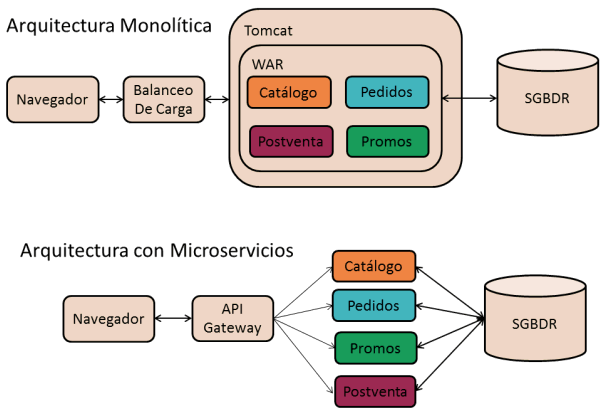
\includegraphics[width=0.7\linewidth]{imagenes/soavsmicroservicios}
		\caption{Monolitica vs Microservicios}
		\label{fig:soavsmicroservicios}
	\end{figure}

	












\section{ ¿Que es un Microservicio?}
	La arquitectura de microservicios pretende dividir una aplicación compleja en pequeños servicios que solo realicen una función especifica y se comuniquen entre ellos para formar la aplicación final.
	
	Cada microservico es una aplicación pequeña totalmente independiente de desarrollar frente al conjunto. Este servicio tiene responsabilidad única, es decir, un único requisito funcional. Ya que este es pequeño, si falla algo es fácil encontrar el error y subsanarlo. 
	
	Ademas al tener un servidor embebido es autoejecutable en cualquier contenedor de aplicaciones, por ejemplo Kubernetes, lo que facilita enormemente su despliegue.
	
	Cada microservicio puede desarrollarse en un lenguaje de programación diferente, gracias a que las peticiones a estos servicios suele ser mediante protocolos ligeros, como HTTP, que son universales a todos los lenguajes de programación. También es fácilmente escalable, se le asignan mas recursos al microservicio que los necesite.
	
	Los expertos en la materia no se ponen de acuerdo en el tamaño que debe tener un microservicio. Sam Newman hace referencia en su libro "Building Microservices"(cita) al experto en microservicios Jon Eaves que el tiempo máximo para desarrollar un microservicio una persona serian dos semanas. Aunque esto es muy relativo, ya que en una empresa grande la funcionalidad que debe realizar cada microservicio no tiene porque ser pequeña, por lo que llevaría mas tiempo.
	
\section{Estado del arte}
	Actualmente la arquitectura basada en microservicios es una realidad y las grandes empresas tales como Netflix, Facebook, Amazon, PayPal se han replanteado la arquitectura que anteriormente usaban para decantarse por los microservicios debido a sus ventajas.

	Rajest RV en su libro "Spring Microservices"\cite{rv2016spring} nos muestra un gráfico en el que se ve como avanza el desarrollo de aplicaciones tradicionales frente a microservicios. "Los microservicios prometen más agilidad, velocidad de entrega y escala. En comparación con las aplicaciones monolíticas tradicionales."
	
	\begin{figure}
		\centering
		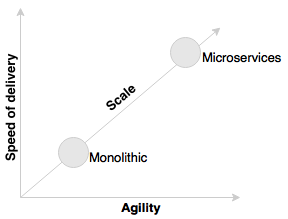
\includegraphics[width=0.7\linewidth]{imagenes/desarrolloMonovsMicro}
		\caption{}
		\label{fig:desarrollomonovsmicro}
	\end{figure}

	Los microservicios han evolucionado tan rápido gracias al desarrollo de nuevas tecnologías. Por ejemplo la creación de bases de datos NOSQL no relacionales, la aparición de docker contenedores de aplicaciones ligeros y portables que facilitan enormemente los despliegues y el comienzo del desarrollo de aplicaciones en la nube. Todo ello unido ha desembocado en la creación de microservicios.
	
	Existen muchas razones por las cuales hacer el cambio o directamente empezar a desarrollar con esta arquitectura. 
	- Los microservicios son mas rápidos y baratos de desarrollar que las antiguas aplicaciones monolíticas. 
	- Es más fácil remplazar una parte de la aplicación global que en los sistemas antiguos. 
	- No necesitas un servidor tipo tomcat donde desplegar la aplicación, ya que cada microserivcio cuenta con uno embebido.
	- Se suelen desplegar en la nube dentro de contenedores dockers por lo que no es necesaria una maquina física(servidor) 24 horas funcionando.
	- Puedes desarrollar cada microservicio en un lenguaje de programación diferente, en función de las necesidades.
	
	Una metáfora que suele usarse para explicar los microservicios es un panal de abeja. Las abejas construyen el panal rellenado pequeñas celdas hexagonales, cada una independiente pero también integrada con las otras. Esto genera una estructura muy fuerte. Si una celda se daña no afecta a las demás, las abejas reconstruyen solo esa celda.
	\begin{figure}
		\centering
		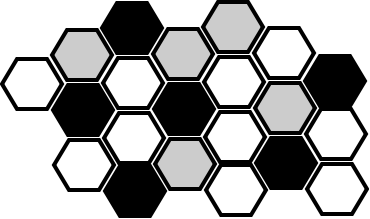
\includegraphics[width=0.7\linewidth]{imagenes/panalAbeja}
		\caption{}
		\label{fig:panalabeja}
	\end{figure}
	
	
	
	


%----------
%	BIBLIOGRAFÍA
%----------	

%\nocite{*} % Si quieres que aparezcan en la bibliografía todos los documentos que la componen (también los que no estén citados en el texto) descomenta está lína

\clearpage
\addcontentsline{toc}{chapter}{Bibliografía}
\setquotestyle[english]{british} % Cambiamos el tipo de cita porque en el estilo IEEE se usan las comillas inglesas.
\printbibliography



%----------
%	ANEXOS
%----------	

% Si tu trabajo incluye anexos, puedes descomentar las siguientes líneas
%\chapter* {Anexo x}
%\pagenumbering{gobble} % Las páginas de los anexos no se numeran



\end{document}